\documentclass[a4paper]{article}
\usepackage[T2A,T1]{fontenc}
\usepackage[utf8]{inputenc}
\usepackage[english, russian]{babel}
\usepackage{graphicx}
\usepackage[hcentering, bindingoffset = 10mm, right = 15 mm, left = 15 mm, top=20mm, bottom = 20 mm]{geometry}
\usepackage{multirow}
\usepackage{lipsum}
\usepackage{amsmath, amstext}
\usepackage{siunitx}
\usepackage{subcaption}
\usepackage{wrapfig}
\usepackage{adjustbox}
\usepackage{enumerate, indentfirst, float}
\usepackage{capt-of, svg}
\usepackage{icomma}

\usepackage[T2A]{fontenc} %кодировка
\usepackage[utf8]{inputenc} %кодировка исходного кода
\usepackage[english,russian]{babel} %локализация и переносы








\newenvironment{bottompar}{\par\vspace*{\fill}}{\clearpage}
 
\begin{document}


\begin{titlepage}
	\centering
	\vspace{5cm}
	{\scshape\LARGE МОСКОВСКИЙ ФИЗИКО-ТЕХНИЧЕСКИЙ ИНСТИТУТ (НАЦИОНАЛЬНЫЙ ИССЛЕДОВАТЕЛЬСКИЙ УНИВЕРСИТЕТ)
 \par}
	\vspace{4cm}
	{\scshape\Large Лабораторная работа №1 \par}
	\vspace{1cm}
	{\huge\bfseries Измерение температуры пламени  \par}
    {\huge\bfseries  методом обращения спектральных линий  \par}
\vspace{1cm}
\begin {figure}[H]
\begin{center}

\includegraphics[width=0.6\textwidth]{faki.png}
\end{center}
\end {figure}
\vspace{1cm}
\begin{flushright}
	{\large выполнили студенты 2 курса группы Б03-104}\par
	\vspace{0.3cm}
	{\LARGE Платонов Никита}\par
    \vspace{0.3cm}
    {\LARGE Алаторцев Кирилл}\par
    \vspace{0.3cm}
    {\LARGE Недопекин Валерий}\par
\end{flushright}
	\vfill
% Bottom of the page
	г. Долгопрудный, 2023 г.
\end{titlepage}


\section*{Аннотация:}
В данной лабораторной работе проводится измерение температуры нагретых тел двумя методами:\par
\begin{enumerate} 
\item методом обращения спектральных линий, с помощью которого определяется температура пламени пропановой горелки,
\item пирометрическим, с помощью которого определяется температура раскаленных металлов
\end{enumerate}
\section*{Цель работы:}
Получить истинную температуры пламени — методом обращения спектральных линий и методом измерения температуры раскалённых металлов с помощью пирометра. И получить поправку к ней.


\vspace{4cm}

%\begin {figure}[H]
%\begin{center}
%\large{ВСЕ КОДЫ К РАБОТЕ МОЖНО НАЙТИ ЗДЕСЬ:}
%\par
%
\includegraphics[width=0.3\textwidth]{qr.png}
%\end{center}
%\end {figure}




\newpage
\section*{Теоретические сведения:}


Среда при любой температуре способна излучать в силу флуктуаций зарядов за счёт теплового движения. Она также способна и поглощать электромагнитное излучение. \par
Спектр излучения занимает широкую область частот — это объясняется большим количеством степеней свобод у частиц таких сред.\par
Далее вводятся основные понятия в теории излучения и законы, описывающие излучение.\par

\begin{enumerate}
    \item Спектральная интенсивность излучения - $I_\lambda dS dt d\lambda d\Omega$ - это величина энергии, переносимая в единицу времени по направлению нормали к единичной площадке в единичном телесном угле.
    \item Считая, что площадка $dS$ расположена непосредственно на поверхности излучающей среды, вводится понятие лучеиспускательной способностью поверхности тела или спектральной поверхностной плотностью излучения в направлении нормали и обозначается $E_\lambda(T)$ как интенсивность излучения с этой поверхности.
    \item В случае диффузного(изотропного) излучения верен закон Ламберта — яркость диффузной поверхности не зависит от направления.
\end{enumerate}

\vspace{0.3cm}

Пусть некое излучение величиной $I_0$ на данной длине волны падает на среду. Тогда возможно несколько процессов, происходящих
с ним в данной среде:

\begin{enumerate}
    \item отражение части падающего излучения - $I^R_0$,
    \item поглощение части проникающего излучения - $I^A_0$
    \item пропускание части проходящего излучения $I^D_0$ .
\end{enumerate}

Тогда с учетом введённых обозначений и закона сохранения
энергии получим:

$$ I^R_0 + I^A_0 + I^D_0 = I_0, $$
или, деля на $I_0$ :
$$ R+A+D=1, $$
где $R, A, D$ – соответственно отражательная, поглощательная и пропускательная способности. \par
Тело, которое при любой температуре полностью поглощает падающее на него излучение произвольной частоты, называется абсолютно черным телом. \par


Далее рассмотрим процесс, в ходе которого устанавливается равновесие между испускаемым и поглощаемым излучением стенками некоторого тела (которые однородны и поддерживаются при постоянной температуре). С учётом сказанного:\par
$$E(T)+R I(T)=I(T) .$$
Внутри полости тела установившееся излучение изотропно и характеризуется величиной, называемой спектральной интенсивностью абсолютно черного тела - $B(T)=I(T)$ . \par
Итого получаем закон Кирхгофа:
$$B(T)= \frac{E(T)}{A(T)}$$
\par
Важно, что отношение лучеиспускательной способности к поглощательной не зависит от вещества и есть спектральная интенсивность черного излучения. \par
При излучении реальных сред вместе с участками спектра, в которых они не излучают, есть такие области, в которых излучение достигает интенсивности черному излучателю, и, такие области, в которых интенсивность излучения составляет часть от интенсивности черного излучения. \par
Величина, характеризующая такие излучатели, называется степенью черноты \par
$$\epsilon (T)=E(T)/B(T).$$
У реального излучения положения максимумов спектральной интенсивностью абсолютно черного тела можно найти из закона Вина:
$$\lambda_{max} T=2.8 * 10^3м*K.$$
Также из определения степени черноты и закона Кирхгофа
видно важное следствие: $\epsilon(T)=A(T)$.



\subsection*{Уравнение интенсивностей излучений пламени и лампы методом обращения спектральных линий:}

\begin {figure}[H]
\begin{center}
\par
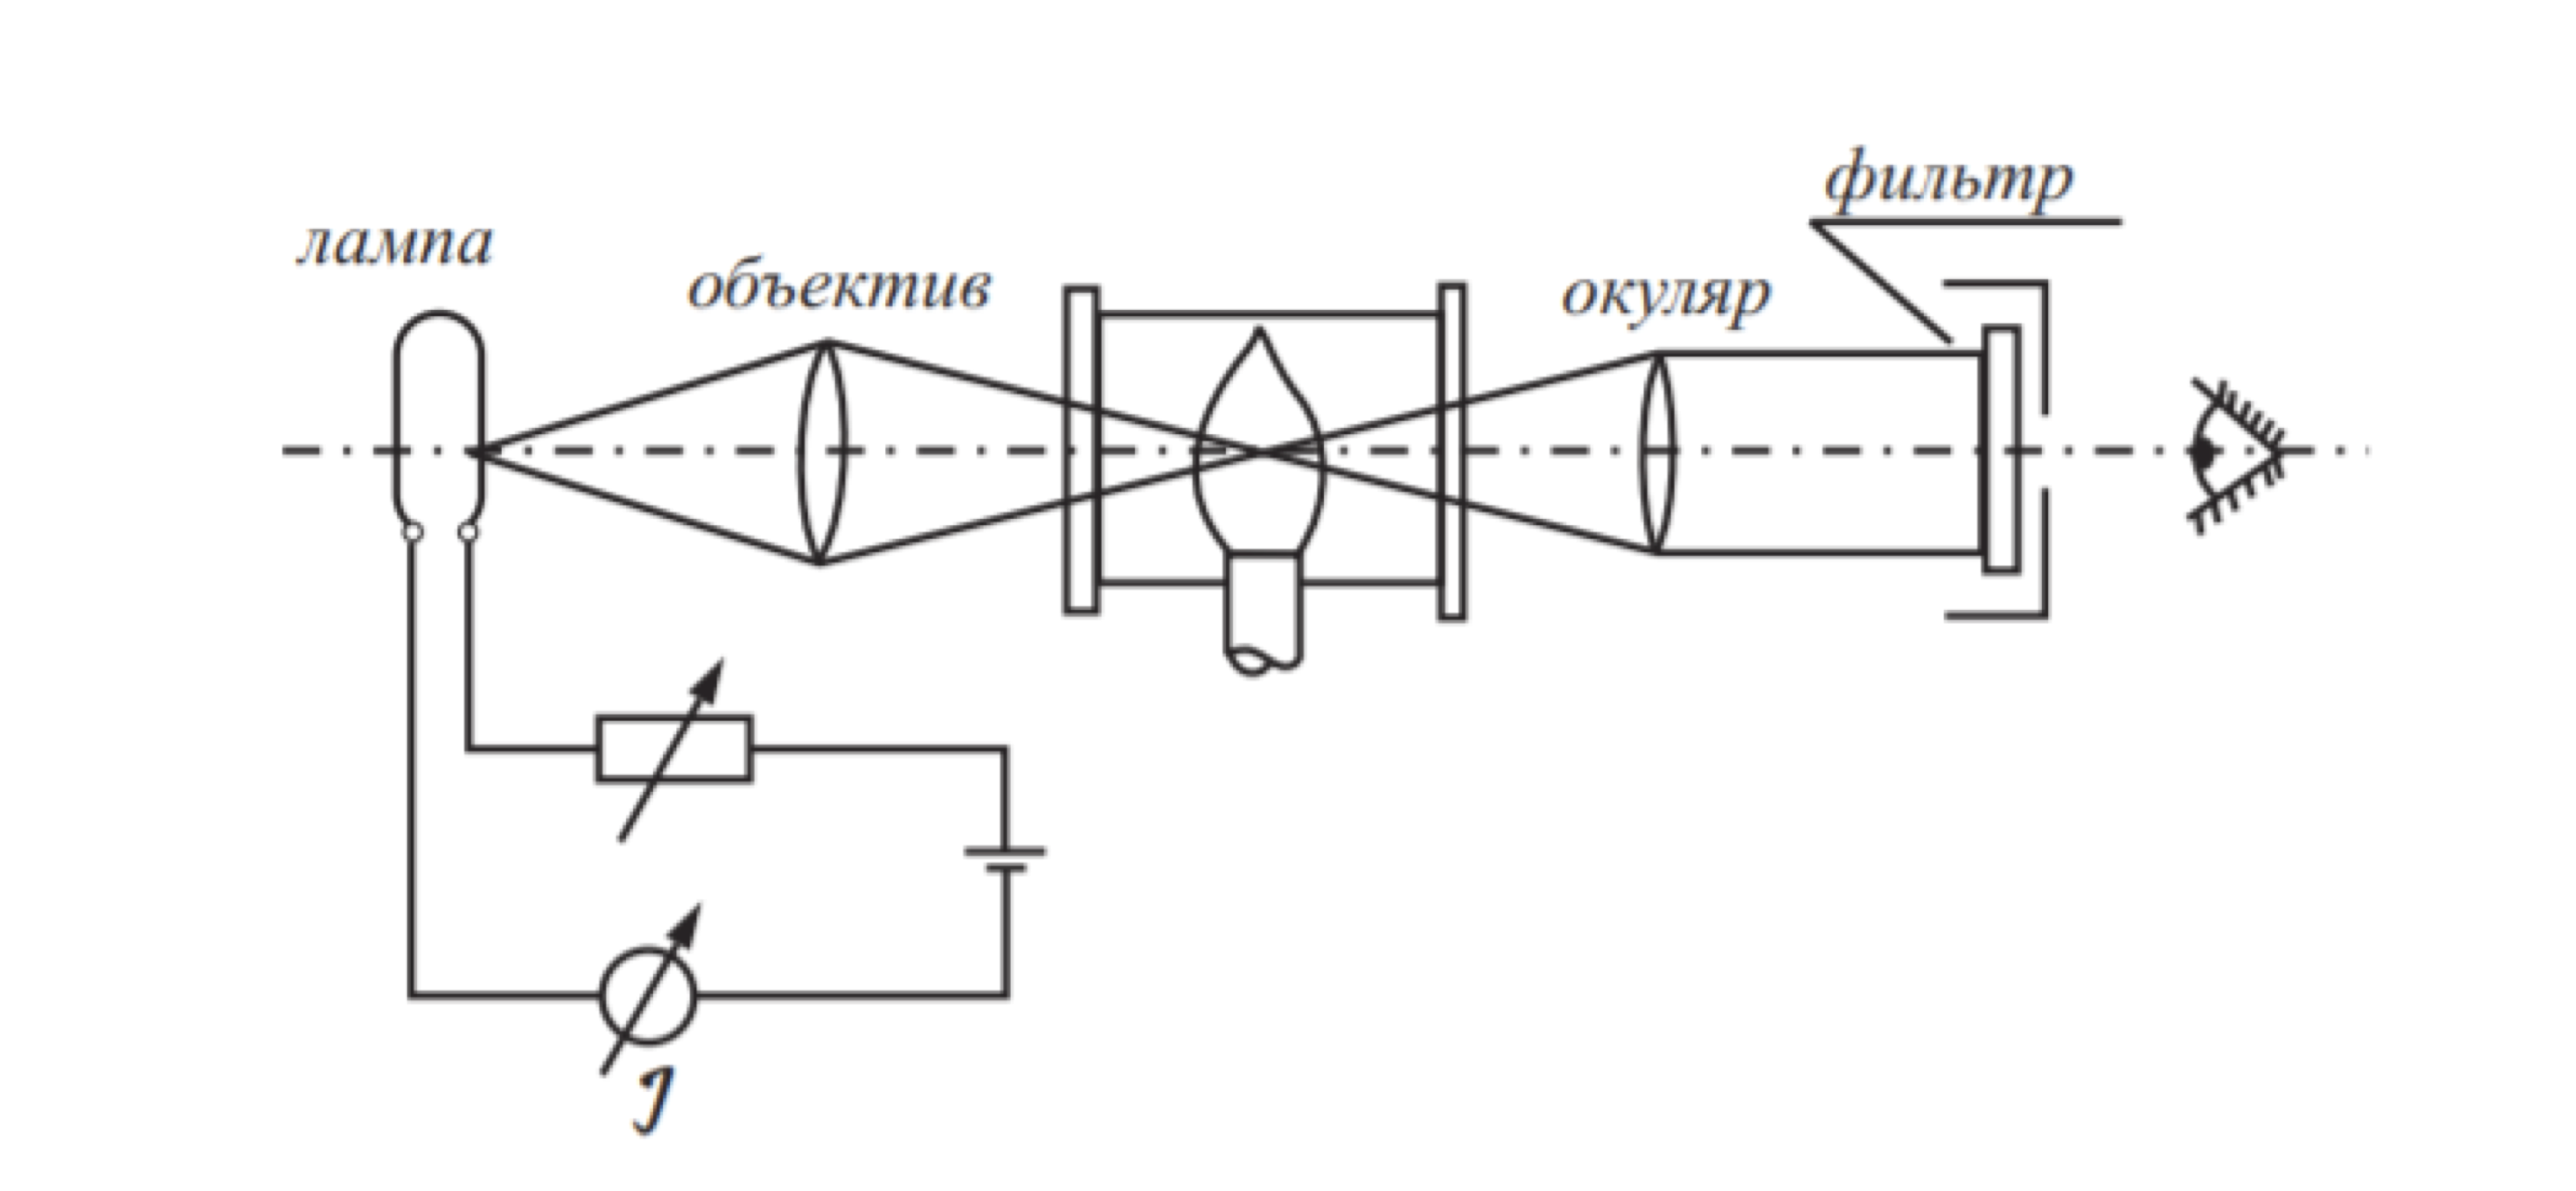
\includegraphics[width=0.9\textwidth]{pl1.png}
\caption{Измерение температуры методом обращения спектральных линий.}
\end{center}
\end {figure}

\par
Нагретые газа обычно являются оптически прозрачными (в большей части спектра — они диатермичны — это связано с отсутствием свободных зарядов), лишь в пределах некоторых полос они могут испускать и поглощать. Поэтому в данном методе мы добавляем примеси, которые по предположению будут находиться в термодинамическом равновесии с газом, отчего они будут излучать в определенном участке видимого спектра (например, мы добавляем натрий — для него известен жёлтый дуплет). \par
В данном методе нужно уравнять интенсивности излучения лампы и пламени, регулируя ток через лампу. Из баланса интенсивностей получим равенство истинной температуры пламени и яркостной температуры лампы. \par
Обычно, вместо фильтра (рис.1) берётся диспергирующий элемент, который разлагает в спектр падающее излучение. В нём видны вертикальные линии, соответствующие спектральным линиям излучения примеси, фон соответствует ленте лампы. \par
Наблюдая данный спектр, мы увеличиваем ток через лампу, отчего яркие вертикальные линии от примесей натрия становятся темнее фона от лампы.  Полученное среднее значение тока - 17,8 А. \par



\begin {figure}[H]
\begin{center}
\par
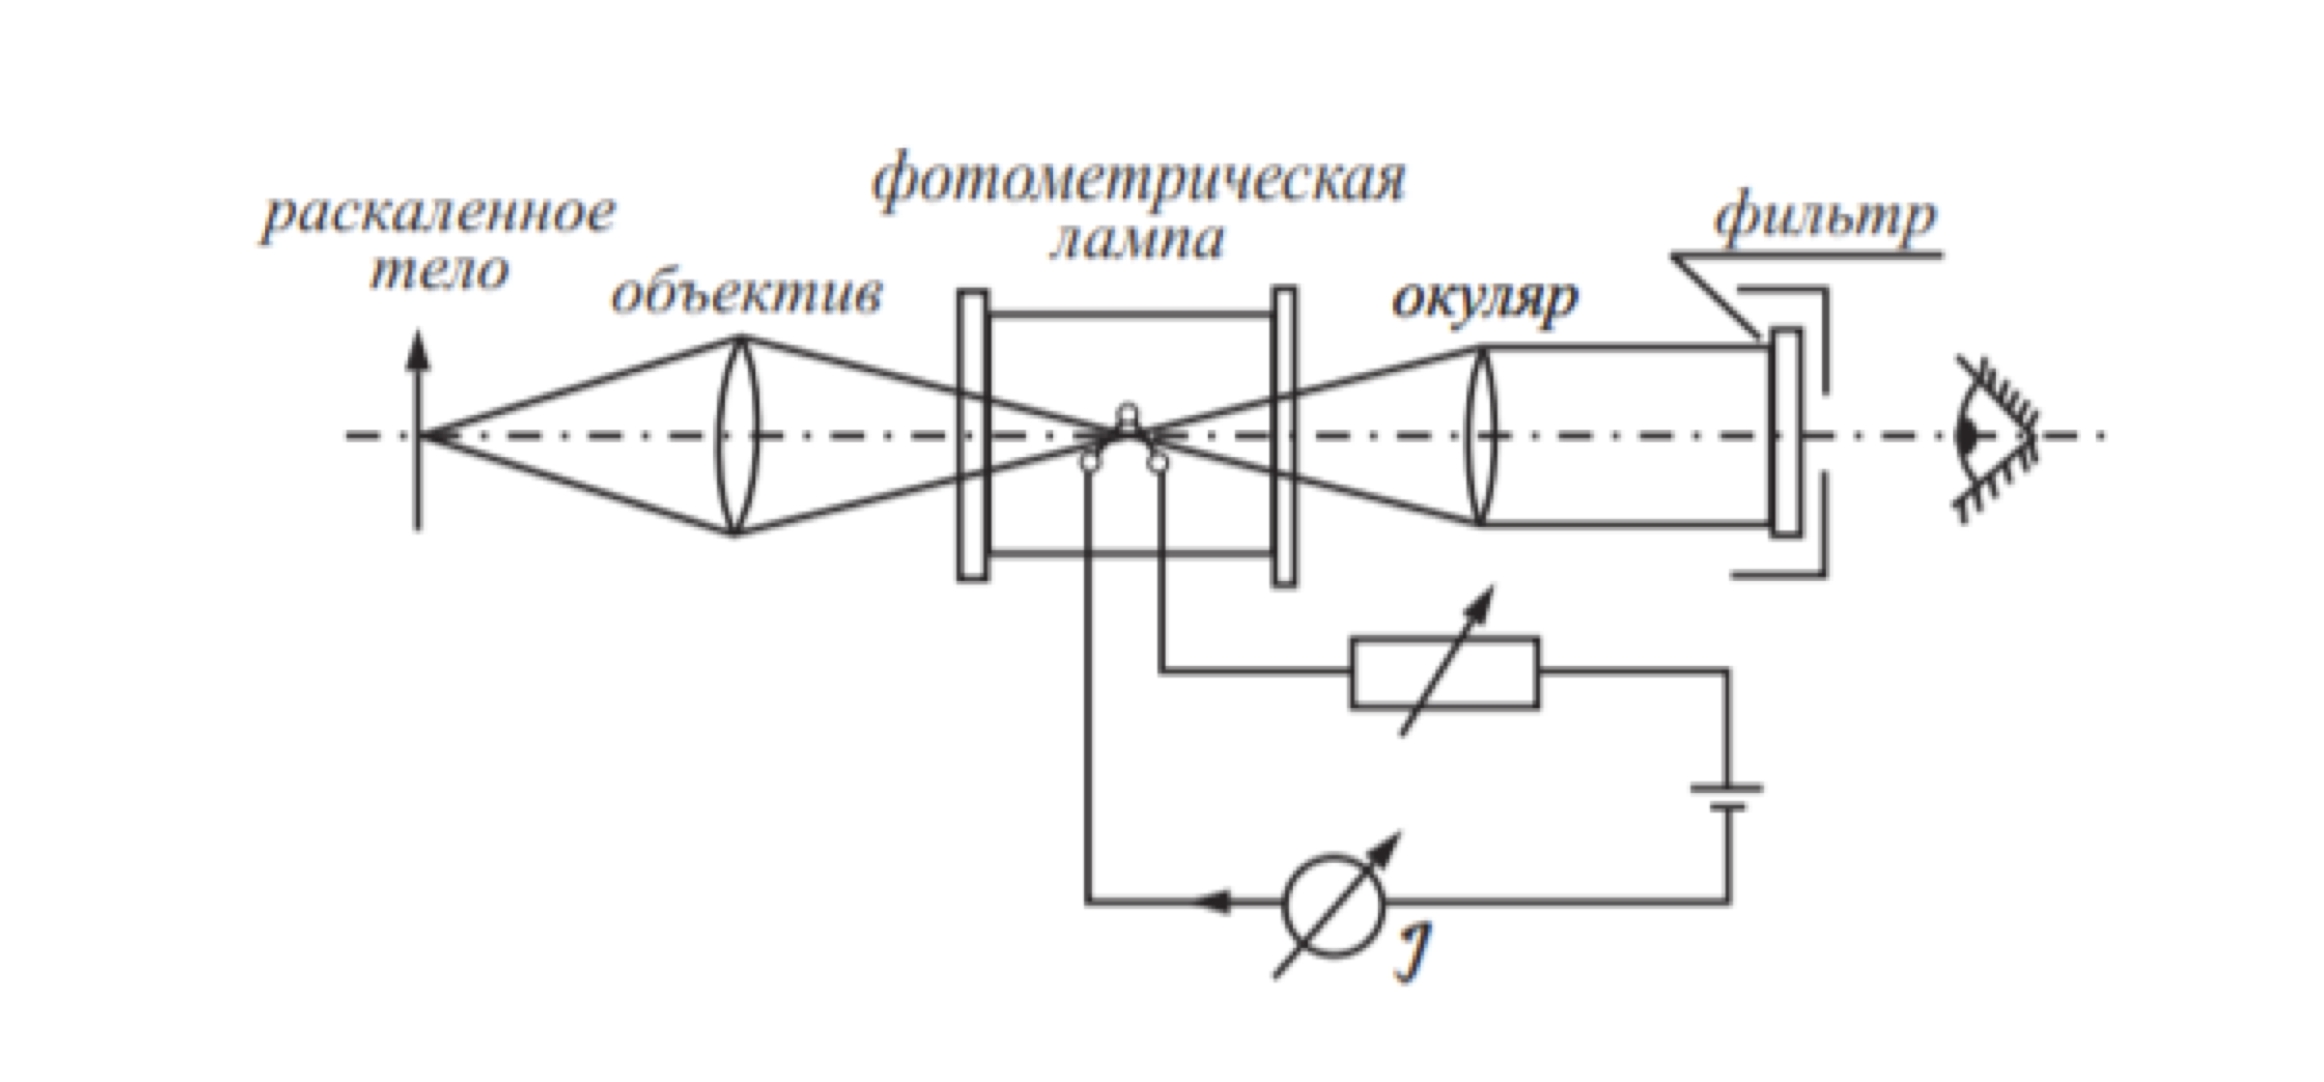
\includegraphics[width=0.9\textwidth]{pl2.png}
\caption{Схема пирометра}
\end{center}
\end {figure}

\par
Для того чтобы измерить температуру раскалённых металлов, существует такие приборы, как пирометры. Работа пирометра основана на сравнении интенсивности света, излучаемого, с одной стороны, объектом, температуру которого измеряют, и, с другой стороны, фотометрической лампой. Однако в силу разных спектральных характеристик объекта и нити пирометра уравнивание интенсивностей происходит в узком участке спектре излучения.
Нить накаливания лампы при этом заранее градуируют, путём сравнения с излучением черного тела (его температуру уже можно померить в широком диапазоне).\par
Опять же, измерение температуры производится через уравнивание интенсивностей:

$$I(T)=B(T_b) $$


Зная функцию B из закона Планка и связь её через степень черноты с функцией $I$, получим формулу для вычисления истинной температуры тела через яркостную $T_k$ , т. к. измеряли её для красного участка спектра: \par

\begin{equation}
        \label{1}
\frac{1}{T_k} + \frac{\lambda_k}{C_2} ln(\epsilon_k) = \frac{1}{T_\text{ж}} + \frac{\lambda_\text{ж}}{C_2} ln(\epsilon_\text{ж}),
\end{equation}


где $C_2 = 1.44*10^{-2}$ K м - константа, известная из закона Планка, $T_\text{ж}$ - истинная температура для желтого дуплета (примеси) (в силу термодинамического равновесия по предположению это и есть искомая температура), $\epsilon_k$=0.4 и $\epsilon_\text{ж}$=0.43 - степени черноты для красного и жёлтого света соответственно,  $\lambda_k$ =650 нм и $\lambda_\text{ж}$=590 нм - длины волн красного и жёлтого света соответственно. \par

Теперь повернём ламп так, чтобы она была обращена к пирометру. Регулируя ток, проходящий через лампу, добьёмся того, чтобы полоса от фотометрической лампы («прямоугольник»), которая сравнена с планемем дуги по интенсивности, слилась с «дугой» от нити пирометра. \par

Полученное значение тока — 69 делений или 347,5 мА.


\begin {figure}[H]
\begin{center}
\par
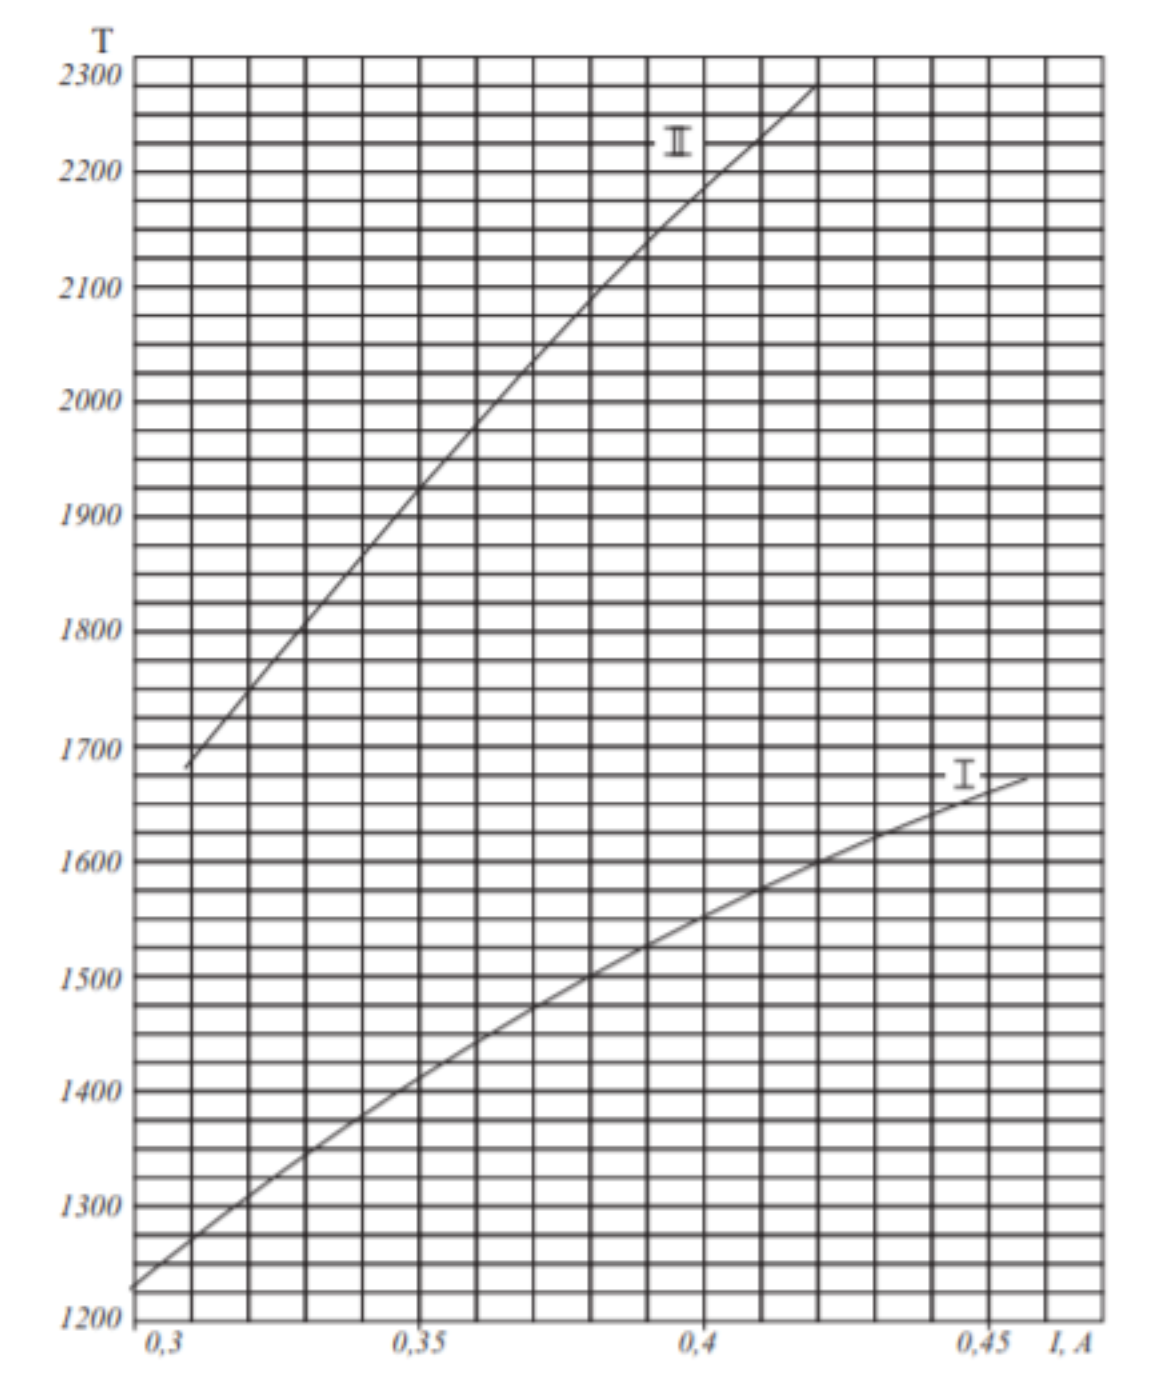
\includegraphics[width=0.75\textwidth]{crivie.png}
\caption{Тарировочные кривые для работы с пирометром.}
\end{center}
\end {figure}

Далее найдём по графику яркостную температуру. $T_k$ = 1925 К. \par

Выразим $T_\text{ж}$ из (1):

$$ T_\text{ж} = \frac{1}{ \frac{1}{T_k} + \frac{1}{C_2} (\lambda_k ln \epsilon_k - \lambda_\text{ж} ln \epsilon_\text{ж}) } $$

Подставляя значения в предыдущую формулу, получаем:

$$ T_\text{ж} = 1950 \text{К}$$ 

\subsection*{Уравнение интенсивностей излучений пламени и лампы методом обращения спектральных линий:}




\section*{Вывод:}
В данном эксперименте было применено два метода для получения истинной температуры пламени — метод обращения спектральных линий и метод измерения температуры раскалённых металлов с помощью пирометра. В ходе первого были уравнены интенсивности фотометрической лампы и пламени, т. е. уравнены яркостная температура лампы и температура пламени. Вторым методом была получена яркостная температура — 1925 К и затем вычислена поправка к ней — 25 К. В итоге в силу физических соображений было получено следующее значение —  1950 К.




\end{document}